%
% some useful macros
%

\newcommand{\CPP}{C\nolinebreak\hspace{-.05em}\raisebox{.4ex}{\tiny\bf +}\nolinebreak\hspace{-.10em}\raisebox{.4ex}{\tiny\bf +}}


\chapter{ \label{chap:modelling} Physics and Detector Modelling}
\writer{F.Gaede, A.Miyamoto}{4}

Accurate and detailed modelling of the physics interactions as well as the detector
response are crucial for making realistic predictions about the expected physics and detector
performance. The ILD software for detector simulation, reconstruction and analysis is entirely
based on the common linear collider software ecosystem called \emph{iLCSoft}~\cite{bib:ilcsoft}.
It will be described in more detail in the next sections.

\section{\label{sec:generator} Modelling of ILC Conditions and Physics Processes}
%
%%\emph{ quick test of hepnames and hepunits:}
%%At $E_{\rm{cms}} = 250~\GeV~$ we cannot measure: $\Pem \Pep \rightarrow \Pqt \Paqt$
%%but of course \Pem \Pep $\rightarrow $ \Pgtm \Pgtp
%%or better write:   \emph{ \Pem \Pep $\rightarrow $ \Pgtm \Pgtp }  ??
%
Large, realistic Monte Carlo samples with the full Standard Model physics ($E_{cms}=500~\GeV$) as well as various
BSM scenarios have been created for the purpose of detector optimization and performance evaluation as
presented in chapter~\ref{chap:performance}. The input samples for the full detector simulation
are created with the Whizard~\cite{Kilian:2007gr} event generator.
Whizard uses tree-level matrix elements and loop corrections to generate events with the final state partons and leptons
based on a realistic beam energy spectrum, the so called \emph{hard sub-process}. The hadronization into the visible final state
is performed with Pythia~\cite{Sjostrand:2006za} tuned to describe the LEP data.
The beam energy input spectrum is created with Guinea-Pig~\cite{Schulte:1998au}, a dedicated simulation program for computing
beam-beam interactions at linear colliders. The two main effects of the strong beam-beam interactions are the energy loss due to
beamstrahlung leading to the available luminosity spectrum (see Fig~\ref{fig:lumi_spectrum}) and the creation of
incoherent $\Pep\Pem$-pairs that are the source of the dominating background at the ILC.
These electrons and positrons are predominantly created in a forward cone as shown in Fig~\ref{fig:lumi_spectrum}. It is this cone that restricts the minimal
allowed radius of the innermost layer of the vertex detector.
%
%%%%%%%%%%%%%%%%
\thisfloatsetup{floatwidth=\textwidth,capposition=below}
\begin{figure}[b!]
\begin{tabular}{cc}
  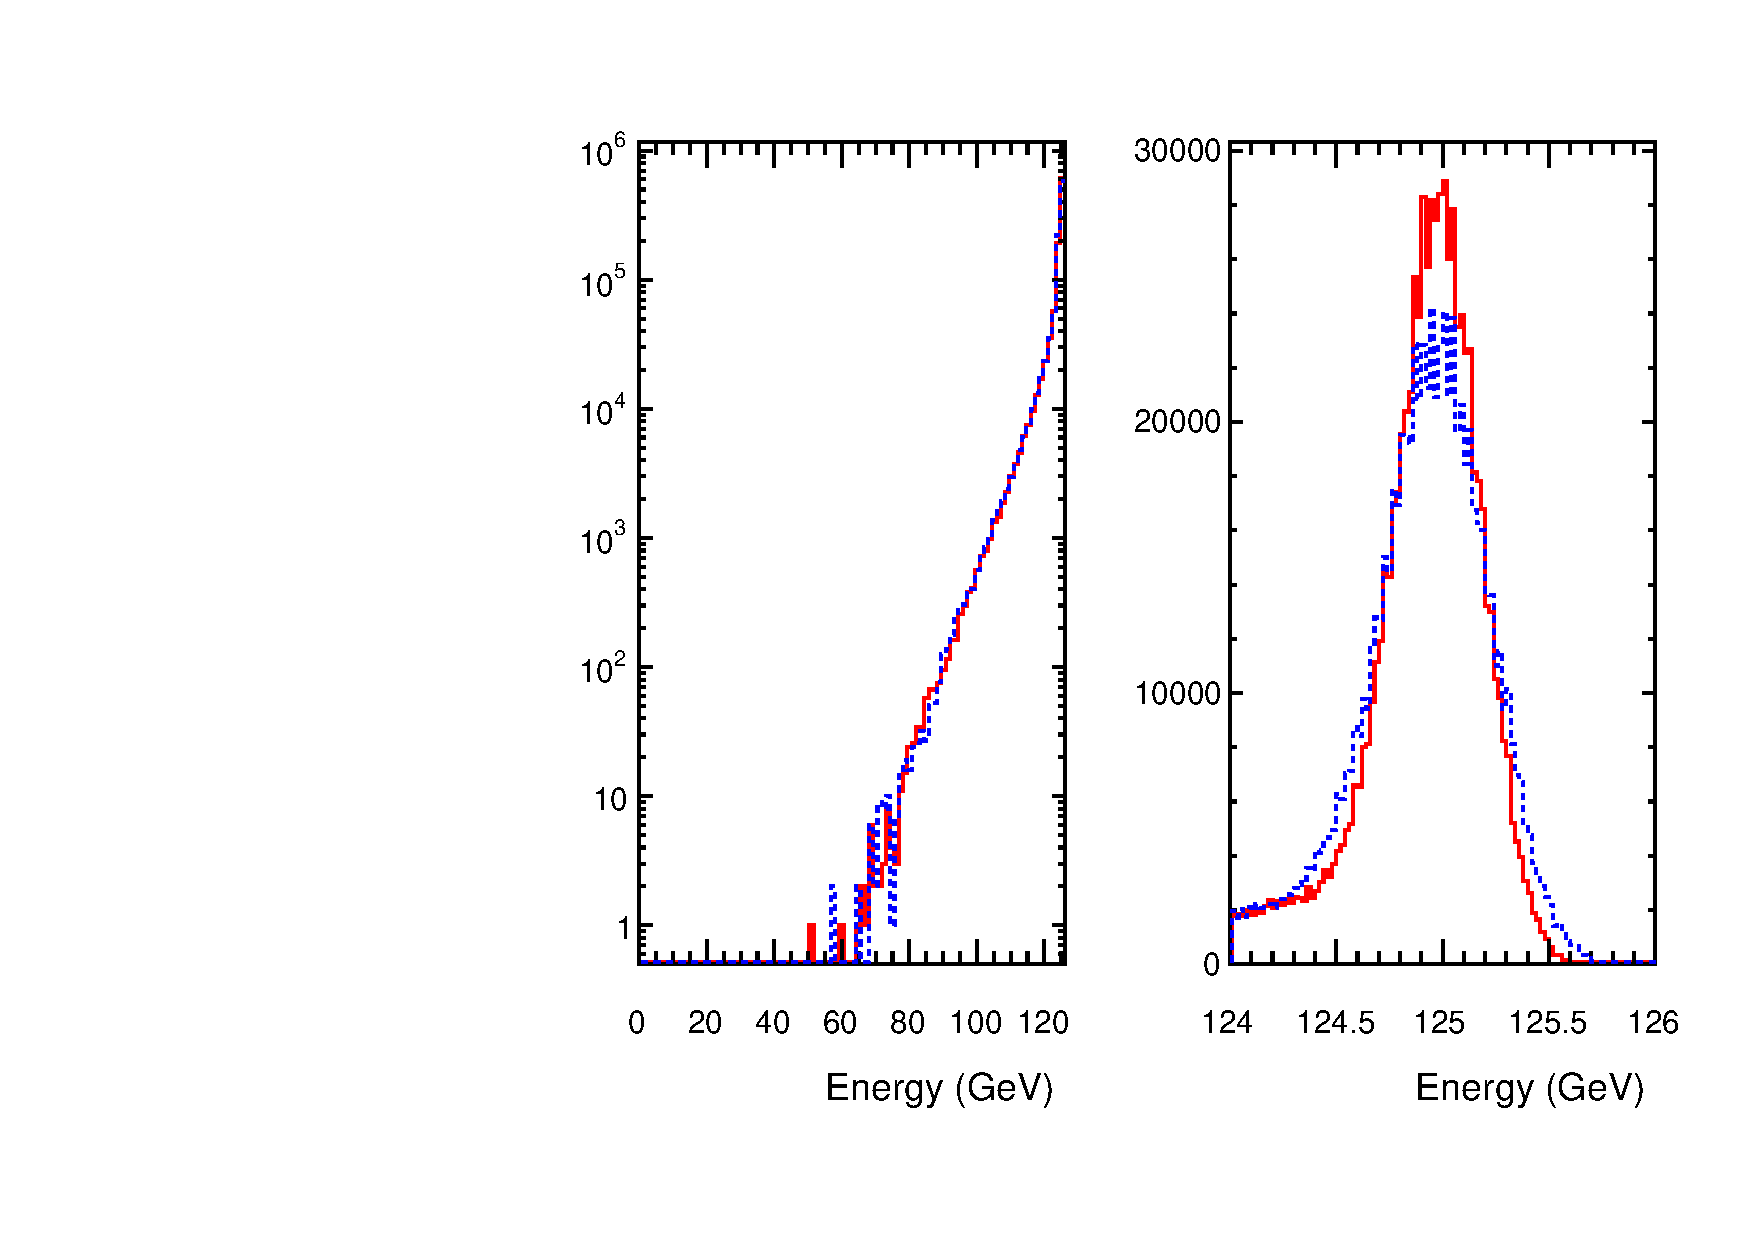
\includegraphics[width=0.51\hsize]{Modelling/fig/beam_spectrum_gp_250Gev_SetA.pdf}
  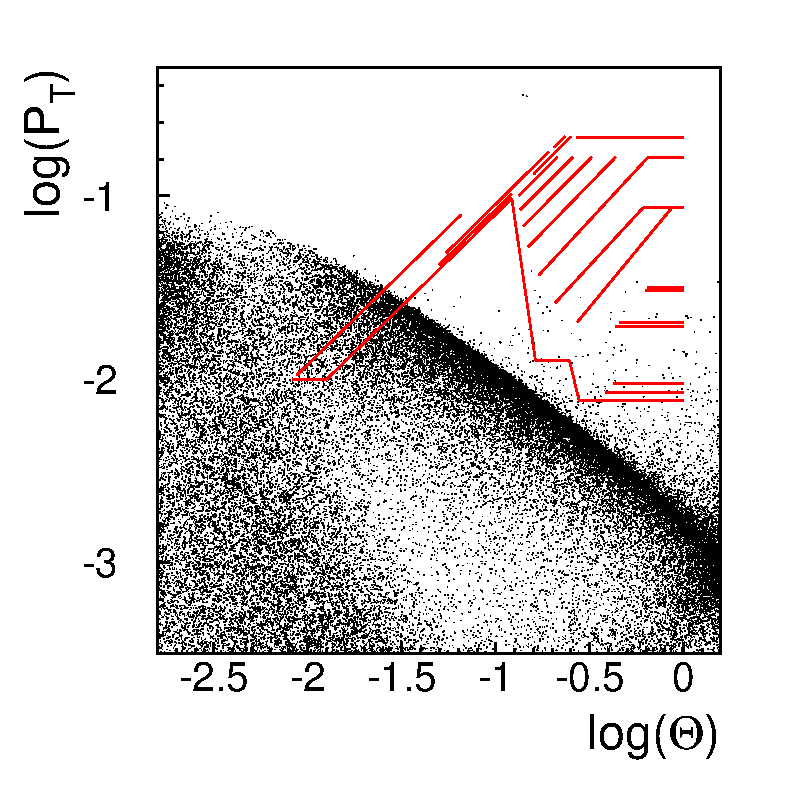
\includegraphics[width=0.49\hsize]{Modelling/fig/gprun_250_SetA_run1_pairs_small.png}
\end{tabular}
\caption{\label{fig:lumi_spectrum}Left: Beam energy spectra for $\sqrt{s}=250~\GeV$ Set-A, created with GuineaPig (blue-dashed:\Pem, red-solid \Pep).
  Right: Cone of incoherent $\Pep\Pem$-pairs in the ILD detector. Shown is $\log{p_t}$, corresponding to the largest radial extend of the
  helical trajectory as a function of $\log{\theta}$. Also shown are the inner detector elements of the ILD detector (horizontal lines represent
  barrel elements and diagonal lines represent end-cap elements).}
\end{figure}
%%%%%%%%%%%%%%%%%
Another source of background at the ILC are $\Pgamma \Pgamma \to hadrons$ events, due to beamstrahlung photons.
These type of events are generated for $\Pgamma \Pgamma$ cms-energies from $300~\MeV ~2~\GeV$ with a dedicated generator based
on ~\cite{Chen:1993dba}, whereas for higher energies Pythia is used.
%
%
For the large Monte Carlo data sets both backgrounds are overlaid to the actual physics event that is simulated. For the incoherent pairs, only
\emph{reconstructable tracks}, i.e. those that leave at least three hits in the tracking detectors, are selected. $\Pgamma \Pgamma \to hadrons$
events are overlaid according to a Poisson-distribution with a total expectation value of $\lambda= 1.1$, resulting from the four
different combinations of the photon virtuality (see table~\ref{tab:ild_aalowpt}).

%-----------------------------------------------------------------------
\begin{table}[htbp]
\renewcommand{\arraystretch}{1.25}

\centering\small
\begin{tabular}{llll}
\hline
process type & Vertex z offset (\micron) & Vertex z sigma (\micron) & expected events per BX \\
\hline \hline
WW &	$0$ 	    &    $196.8$          &     $0.211$  \\
WB &	$- 42.22$    &   $186.0$          &     $0.246$  \\
BW &	$+ 42.22$    &   $186.0$          &     $0.244$  \\
BB &	$0$ 	    &    $169.8$          &     $0.351$  \\
\hline
\end{tabular}
\caption{Key parameters used in the overlay of $\Pgamma \Pgamma \to hadron$ background at $\sqrt{s}=500~\GeV$ for the four different combinations of photon
  virtualities. W denotes a virtual photon and B a real photon.\label{tab:ild_aalowpt} }
\end{table}
%-----------------------------------------------------------------------


\section{\label{sec:det-sim} Detector Simulation}

The main core software tools in iLCSoft used by ILD are the common event data model and persistency tool LCIO~\cite{Gaede:2003ip}
and the \CPP\ application framework Marlin~\cite{Gaede:2006pj} and the recently added generic detector description toolkit
DD4hep~\cite{Frank:2014zya,Frank:2015ivo}. DD4hep provides a single source of information for describing the detector geometry, its
materials and the readout properties of individual sub detectors. Various components of DD4hep provide different functionality.
Here we use DDG4, the interface to full simulations with Geant4~\cite{Agostinelli:2002hh} and DDRec the specialized view into the
geometry needed for reconstruction.
%
%%% conditions data and alignment with DDCond and DDAlign respectively, see Fig.~\ref{fig:dd4hep}.
%%% %%%%%%%%%%%%%%%%
%%% \thisfloatsetup{floatwidth=\SfigwFull,capposition=beside}
%%% \begin{figure}[b!]
%%% 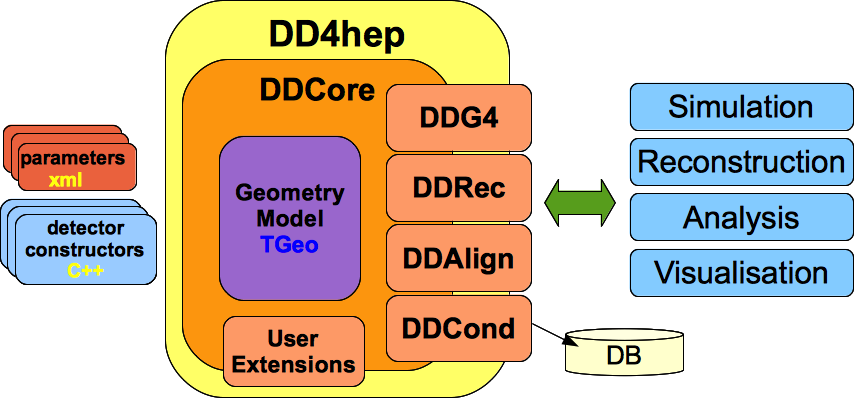
\includegraphics[width=0.7\hsize]{Modelling/fig/dd4hep_simple_schema.png}
%%% \caption{\label{fig:dd4hep}Schematic view of DD4hep and its main components.}
%%% \end{figure}
%%% %%%%%%%%%%%%%%%%%
\thisfloatsetup{floatwidth=\textwidth,capposition=below}
\begin{figure}[b!]
\begin{tabular}{cc}
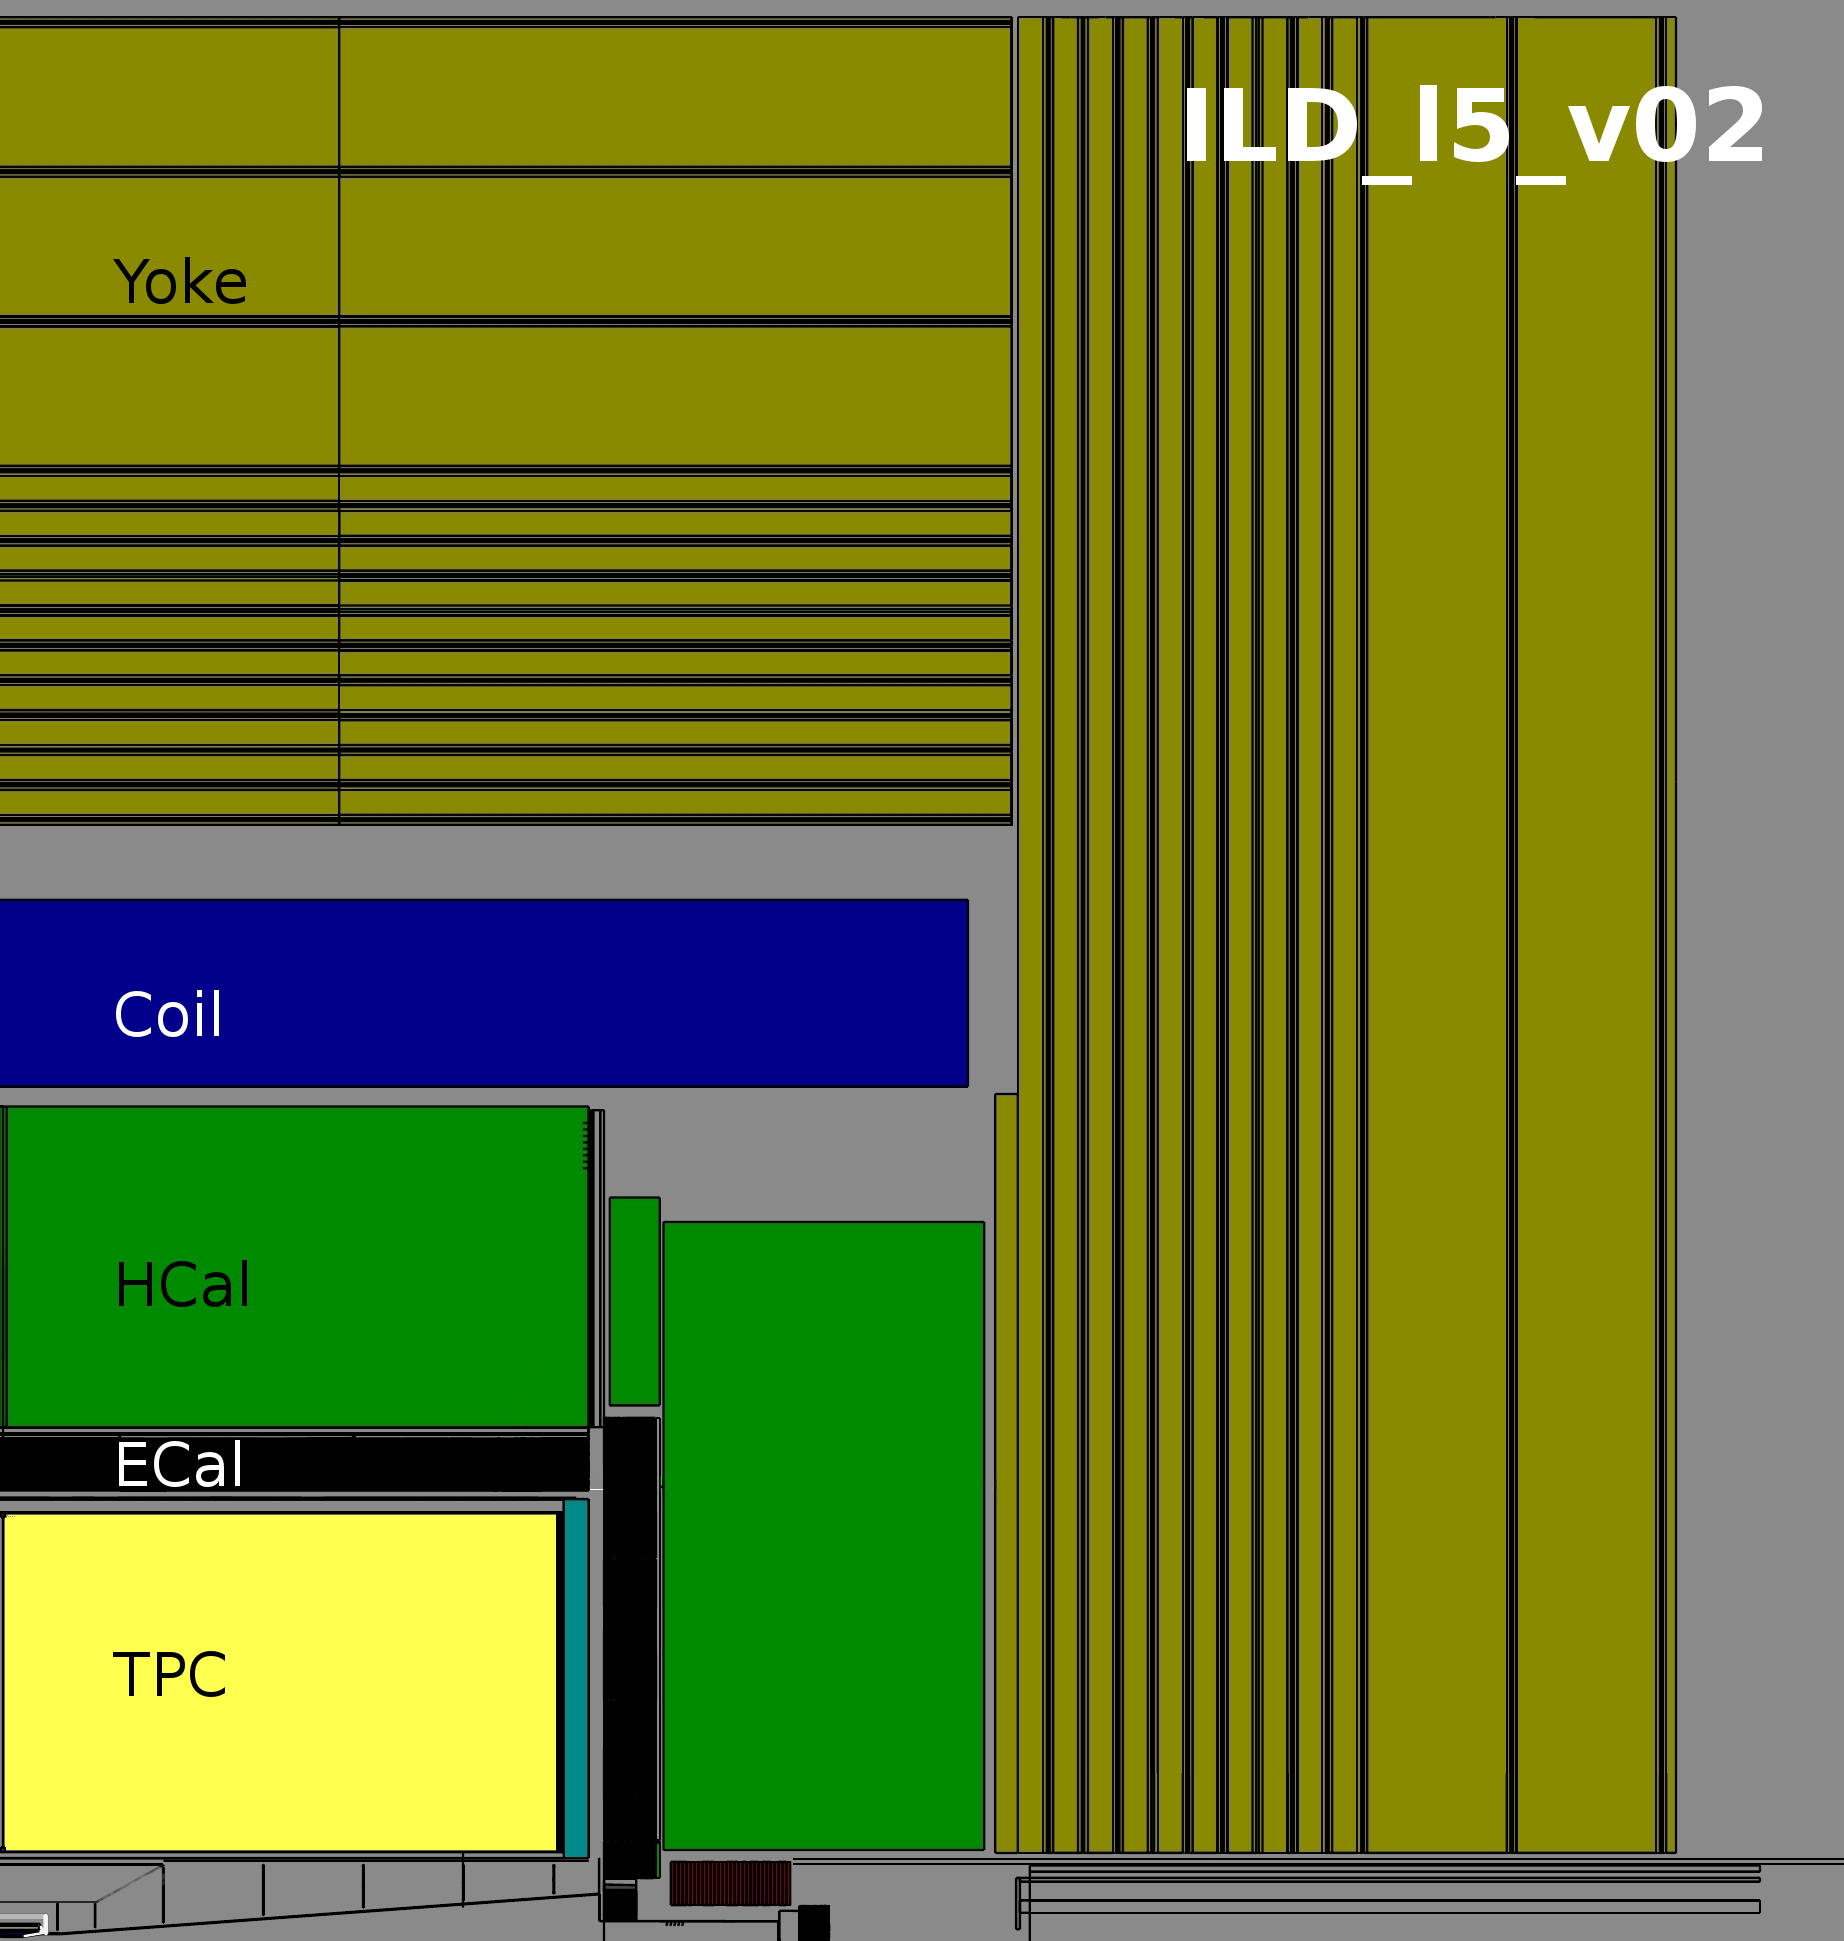
\includegraphics[width=0.45\hsize]{Modelling/fig/ILD_l5_v02_sideview_gimp_2.jpg}
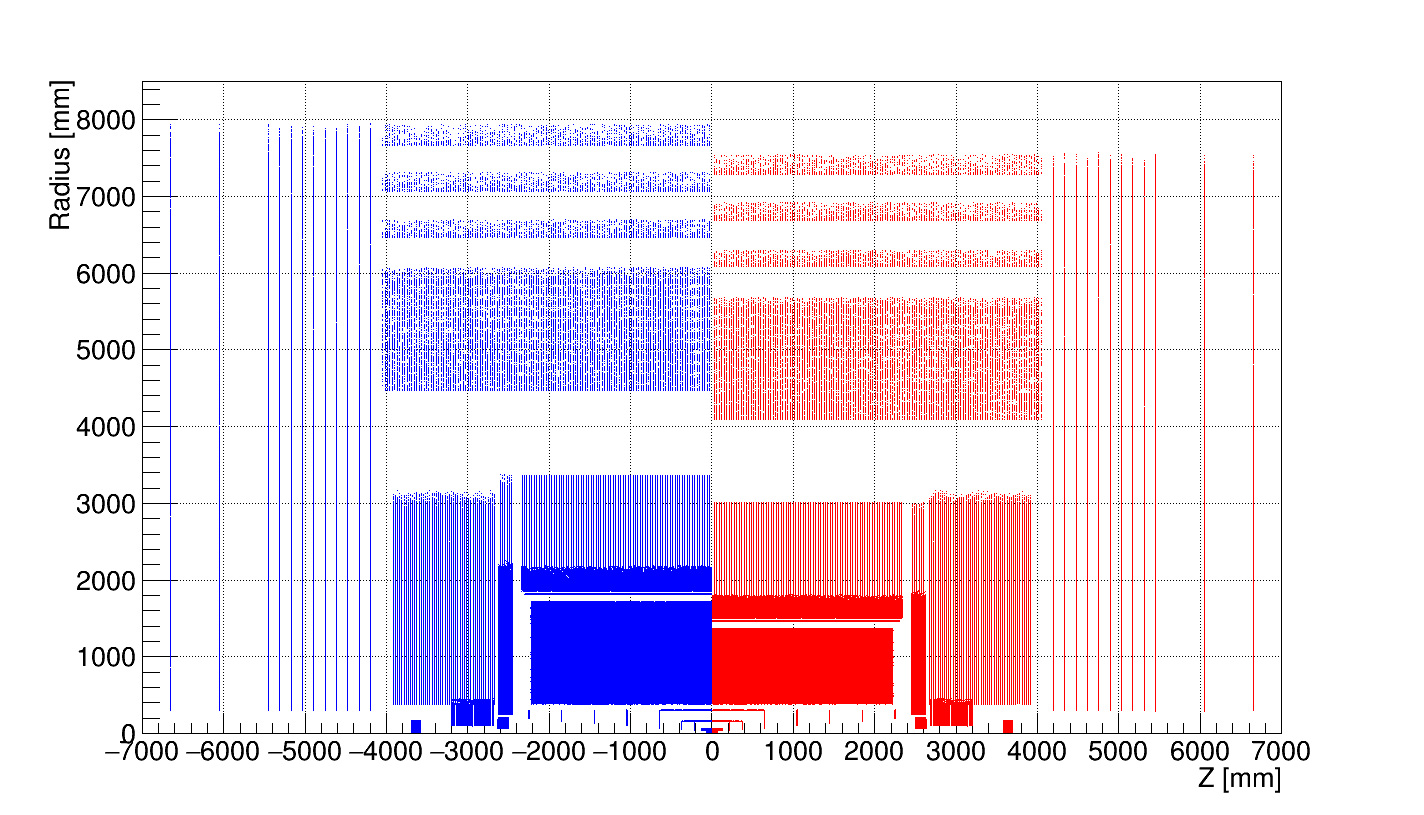
\includegraphics[width=0.55\hsize]{Modelling/fig/hits_rz_small_large_ILD.png}
\caption{\label{fig:sim_model_quad}Left: Quadrant view of the (large) ILD simulation model. Not labeled in the figure are the inner
  silicon tracking detectors: VXD, SIT and FTD, the outer silicon tracker SET as well as the forward calorimeters LCal, LHCal and BeamCal.
  Right: Simulated hits in the large and small ILD simulation models in the $rz$-view.
}
\end{tabular}
\end{figure}


\subsection{\label{sec:det-models} ILD Simulation Models}

For detector optimization studies two ILD simulation models: \emph{ ILD\_l5\_v02} (large)
and \emph{ ILD\_s5\_v02} (small) with the dimensions described in tables~\ref{ild:tab:barrelpara} and~\ref{ild:tab:endcappara},
have been implemented using DD4hep and released in a dedicated software package: lcgeo~\cite{bib:lcgeo}.
A quadrant view of the large simulation model is shown in Fig.~\ref{fig:sim_model_quad} together with a plot of simulated
hits in the large and small detector model for comparison. The main difference between the two models are the reduced radii of
the TPC, the barrels of Ecal, Hcal, Yoke and the Coil. All other detector dimensions including all material thicknesses have not been modified.
%
Considerable effort has been invested into making the ILD simulation models as realistic as possible, in particular by
\begin{itemize}
\item following the exact dimensions and layout of detector elements from engineering models
\item implementing correct material properties
\item implementing precise descriptions of the actual detector technology
\item adding realistic amounts of dead material from supports and services, such as cables and cooling pipes
\item introducing realistic gaps and imperfections into the subdetectors
\end{itemize}
Care has been taken to include realistic material estimates in particular in the tracking region where
the material budget has a direct impact on the detector performance. 
Fig.~\ref{fig:sim_large_small}-left shows the  material budget in the ILD tracking volume resulting from the
individual tracking subdetectors including dead material and services. The spike at the edge of the tracking
fiducial volume at $\theta \approx 5^{\circ}$ is due to the shallow crossing of cables routed along the
conical part the beam pipe. Fig.~\ref{fig:sim_large_small}-right shows the material distribution in the
inner tracking region close to the IP.

%%as well as simulated tracker and calorimeter hits for the large and small model respectively.

%%%%%%%%%%%%%%%%
\thisfloatsetup{floatwidth=\textwidth,capposition=below}
\begin{figure}[b!]
\begin{tabular}{cc}
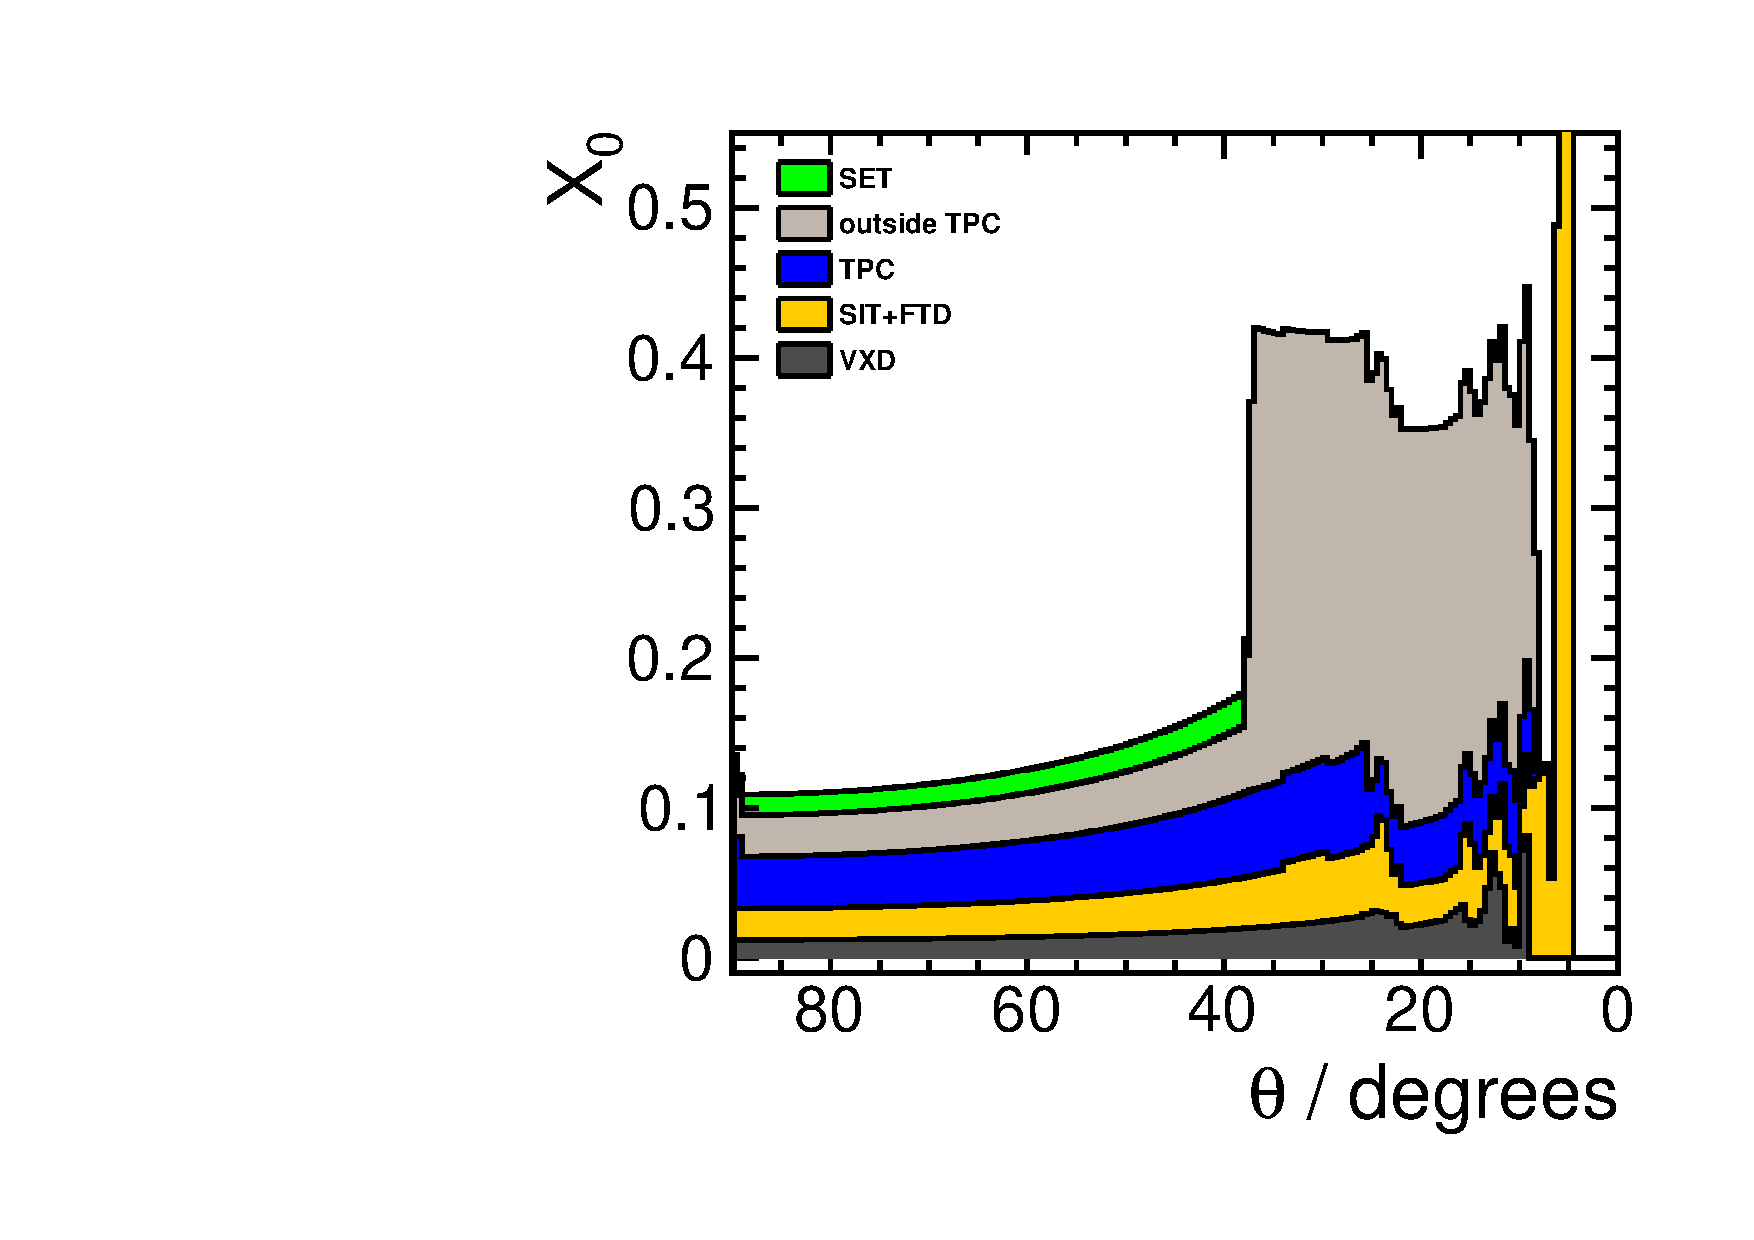
\includegraphics[width=0.4\hsize]{Modelling/fig/ILD_l5_v02_matbudget_tracker_85deg.pdf} &
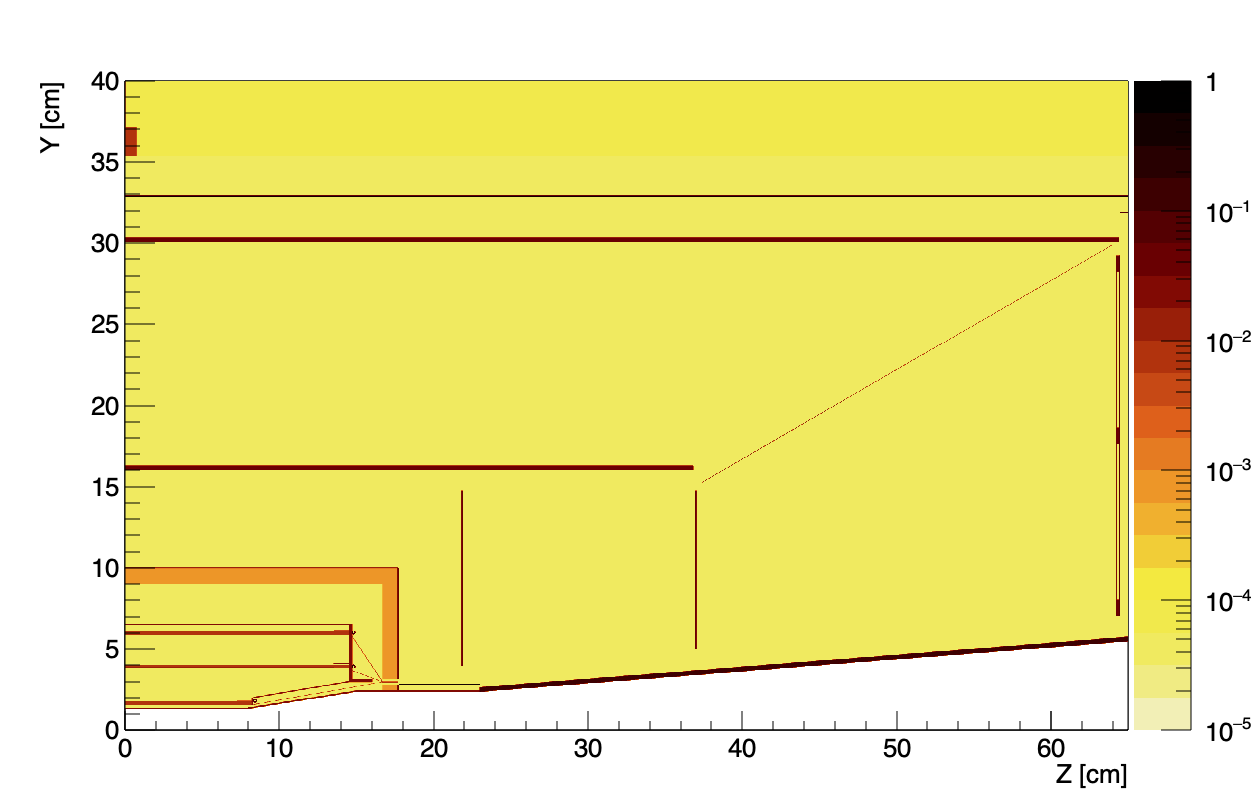
\includegraphics[width=0.6\hsize]{Modelling/fig/ILD_large_inner_tracker_x0_scan.png}
\end{tabular}
\caption{\label{fig:sim_large_small}Left: Integrated radiation lengths of the tracking detectors in the ILD simulation models.
  Right: Material scan in inner tracking region of the simulation model (inverse X0 in arbitrary units) showing detector components of the VXD, SIT and FTD as well
  as dead material from the beam pipe, support structures, cables and services.}
\end{figure}
%%%%%%%%%%%%%%%%%


\subsection{Hybrid Simulation}

In order to be able to study and compare the different calorimeter technologies proposed for ILD
(see chapter~\ref{ild:sec:HCAL}) \emph{hybrid simulation} models have been implemented for the
ILD simulation models, where two different readout technologies are implemented in the
gaps of the sandwich absorber structure as shown in Fig.~\ref{fig:hybridsim}~(right). 
%
%%%%%%%%%%%%%%%%
\thisfloatsetup{floatwidth=\SfigwFull,capposition=beside}
\begin{figure}[b!]
\begin{tabular}{cc}
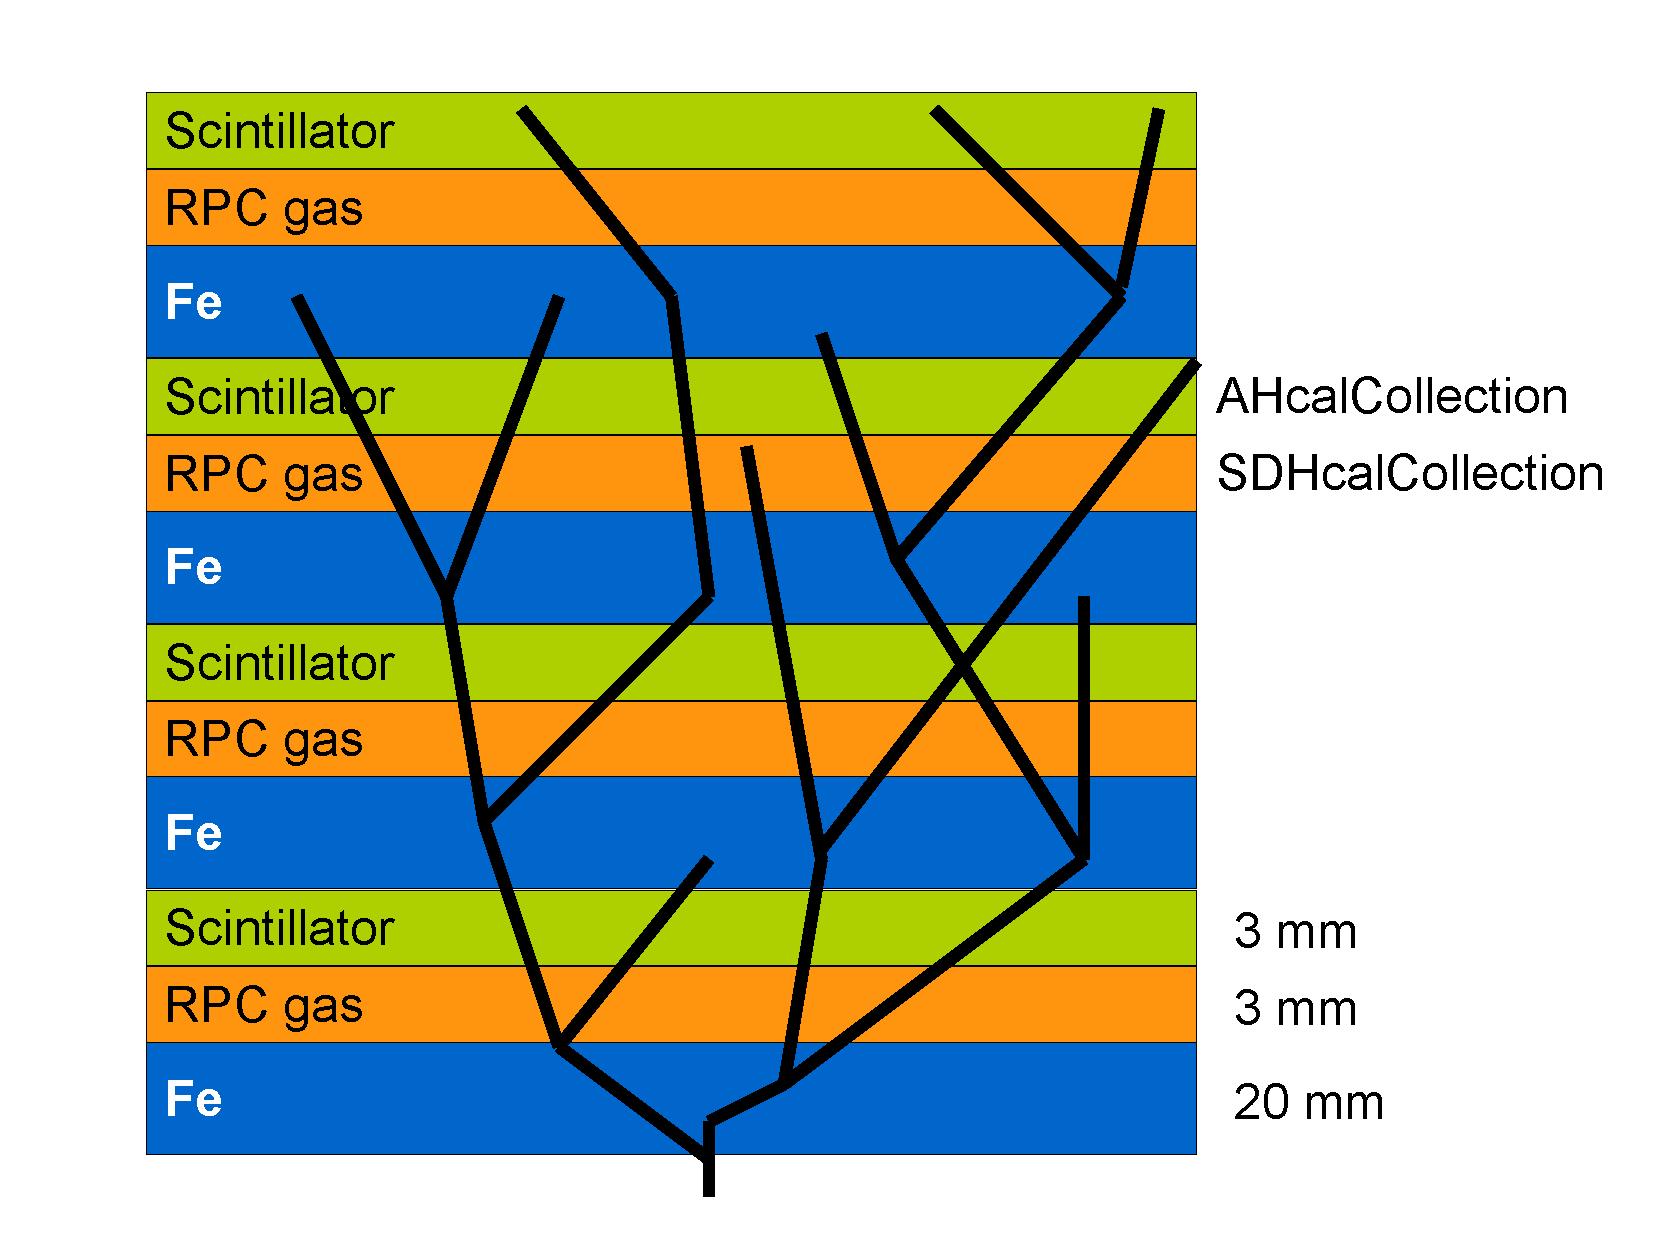
\includegraphics[width=0.5\hsize]{Modelling/fig/multi_technology_simulation.pdf}  &
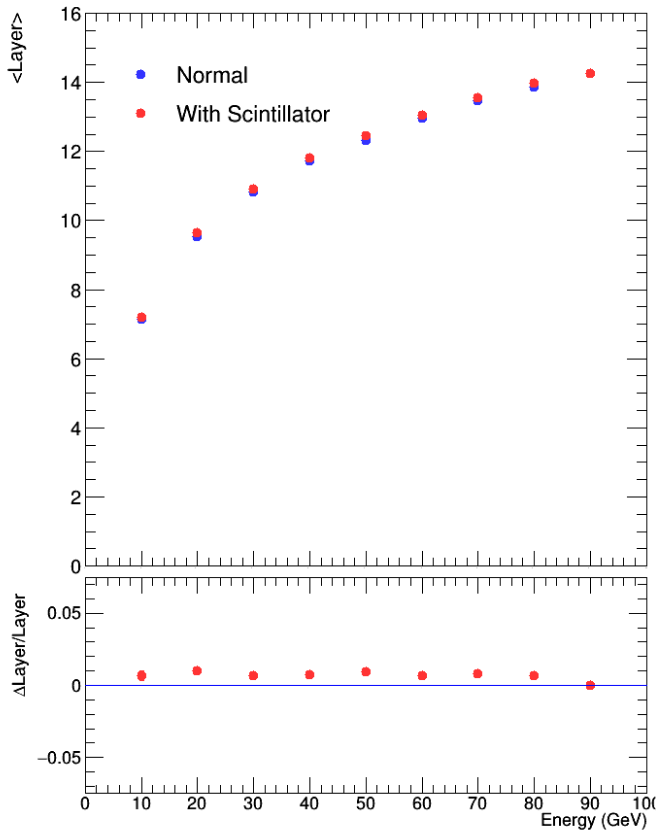
\includegraphics[width=0.5\hsize]{Modelling/fig/SDHcal_hybrid_normal_comparison.png}
\end{tabular}
\caption{\label{fig:hybridsim}Left: Schematic view of the \emph{hybrid simulation} model for two different
  calorimeter technologies using scintillator and RPCs respectively.
  Right: Longitudinal shower profile for the individual simulation of the RPCs (\emph{normal}) compared to
  the hybrid simulation (\emph{with scintillator}).}
\end{figure}
%%%%%%%%%%%%%%%%%
As the calorimeter shower development is almost entirely dominated by the absorber structure, this approach
provides results that are equivalent to the stand alone simulation of each individual technology to better than 1\%,
as shown in Fig.~\ref{fig:hybridsim}~(left) for the longitudinal shower profile. Equivalent results have
been obtained for other parameters, such as the total number of hits and the transverse shower profile.
With this approach one can simulate a large set of Monte Carlo events for
several calorimeter technologies using only little more CPU time than would be needed for simulating just one
technology choice and at the same time one can compare different technologies with identical physics events.


\section{\label{sec:reco} Event Reconstruction}
The detailed simulation with Geant4 provides hit objects with the exact amount and position of energy
depositions in individual sensitive detector elements, such as silicon pixels or calorimeter cells.
In the \emph{Digitization} step all relevant effects from the detector technology and the readout electronics
are applied to the simulated hits.

\subsection{Digitization}
For silicon strip-and pixel detectors as well as the ILD-TPC, the hit positions are smeared according to
resolutions that have been established from test beam campaigns for the different sensor technologies,
thereby including effects from charge sharing, clustering and position reconstruction.
Table~\ref{tab:ild_trk_res} shows the point resolution parameters used in the current ILD simulation models.
%
%-----------------------------------------------------------------------
\begin{table}[htbp]
\renewcommand{\arraystretch}{1.25}

\centering\small
\begin{tabular}{llcl}
\hline
 Subdetector &  \multicolumn{3}{c}{ Point Resolution }  \\
\hline
        VTX    &  $ \sigma_{r\phi,z}  $  & $=$ &  \unit{3.0}{\micron} (layers 1-6) \\
        SIT    &  $ \sigma_{r\phi,z}  $  & $=$ &  7.0~\micron (layers 1-4) \\

        SET    &  $ \sigma_{\alpha_{z}}$  & $=$ &  7.0~\micron  (layers 1-2)  \\
               &  $  \alpha_{z}      $  & $=$ &   $ \pm \unit{7}{^\circ} $ (angle with z-axis)  \\

       FTD     &  $\sigma_{r}$         & $=$ & 3.0~\micron   (layers 1-2) \\
  \emph{Pixel} &  $ \sigma_{r_\perp}$   & $=$ & 3.0~\micron    \\

     FTD       &  $ \sigma_{\alpha_r}   $ & $=$ &  7.0~\micron  (layers 3-7)   \\
  \emph{Strip} &  $ \alpha_{r}         $ & $=$ & $\pm \unit{5}{^\circ} $ (angle with radial direction)        \\

       TPC    &  $ \sigma^2_{r\phi} $ & $=$ & $ \bigl( 50^2+900^2\sin^2\phi + \bigl( (25^2/22)\times$  \\
              &                      &     &   $(4~\rm{T}/B)^2\sin\theta\bigr) (z/\cm) \bigr)\,\micron^2$  \\
               &  $ \sigma^2_{z}    $ & $=$ & $ (400^2+80^2\times (z/\cm)) \,\micron^2 $ \\
               &   \multicolumn{3}{c}{ where $\phi$ and $\theta$ are the azimuthal and} \\
               &   \multicolumn{3}{c}{ polar angle of the track direction } \\
\hline
\end{tabular}
\caption[Simulated ILD tracking point resolutions.]{Effective point resolutions as used in the digitization of
  the ILD tracking detectors.
  The parameterization for the TPC takes into account geometric effects due to the direction of the track with
  respect to the pad row and
  has been established from test beam data.
        \label{tab:ild_trk_res} }
\end{table}
%-----------------------------------------------------------------------
In the TPC hit digitization, simulated hits that are closer than the established double-hit resolution
of 2~mm in $r\phi$ and 5~mm in $z$ are merged into one.
For the silicon detectors this treatment is not necessary, due to the expected low occupancies.
During the calorimeter digitization a two step calibration is applied for every calorimeter type and
sampling structure. In a first step the hits are calibrated to a MIP signal and in a second step,
the total energy is calibrated to an absolute value of the cell energy in \GeV.
This calibration is an iterative procedure, based on the application of the full
\emph{particle flow algorithm } to single particle events with \Pphoton and \PKz and thereby
repeatedly adjusting the calibration constants.
%\fix{reference for calibration procedure ?}
For scintillating calorimeters Birk's Law, resulting in different light yields for different
particles, is already applied during the simulation. Dedicated digitizers take into account
effects of non-uniformity of the light yield for scintillators as well as cross-talk between
neighboring channels.

\subsection{Track reconstruction}

The ILD track reconstruction is described in more detail in~\cite{Gaede:2014aza}. The \emph{pattern recognition}
step is carried out independently in three regions:
\begin{itemize}
\item inner Si-trackers  VXD and SIT ( and partly FTD)\\
  brute-force triplet seeding followed by a road search using extrapolations to the next layer
\item forward Si-tracker: FTD \\
  a Cellular-Automaton finding many track candidates; reduced to a unique and consistent set through the use of a Hopfield Network.
\item the TPC \\
  topological clustering in the outer TPC pad row layers for seeding, followed by a Kalman-Filter based road search inwards
\end{itemize}
In a final step the track candidates and segments are combined into a unique set and then, after assignment of left-over hits, a final
refit is performed with a Kalman filter.
%
The correct reconstruction of the kinematics of charged particles requires a sufficiently detailed description of the material
the particles have traversed, in order to correctly account for effects of energy-loss and multiple-scattering in the fit.
The DD4hep component DDRec provides dedicated surface classes for track reconstruction and fitting. These surface classes provide the
geometric information of the corresponding measurement surfaces as well as material properties, averaged automatically from
the detailed model. Surfaces are also used to account for effects from dead material layers, such as support structures or cables and services.
Fig.~\ref{fig:inner_trk_surfaces} shows the tracking surfaces used for the inner tracking detectors of ILD.
%
%%%%%%%%%%%%%%%%
\thisfloatsetup{floatwidth=\SfigwFull,capposition=beside}
\begin{figure}[b!]
\begin{tabular}{cc}
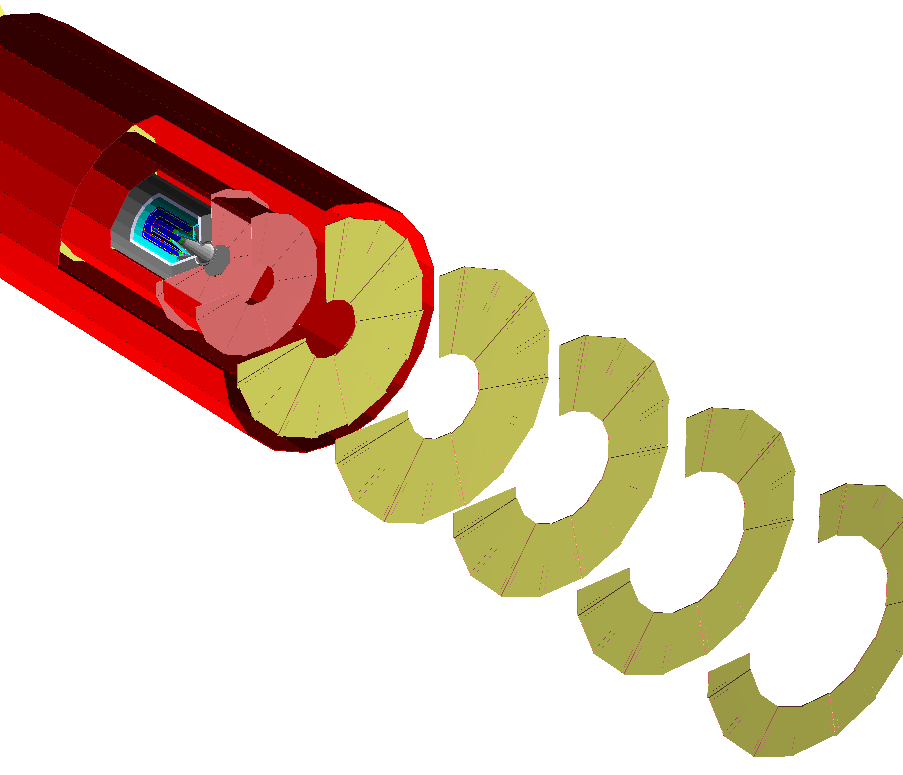
\includegraphics[width=0.5\hsize]{Modelling/fig/ild_inner_trackers.png} &
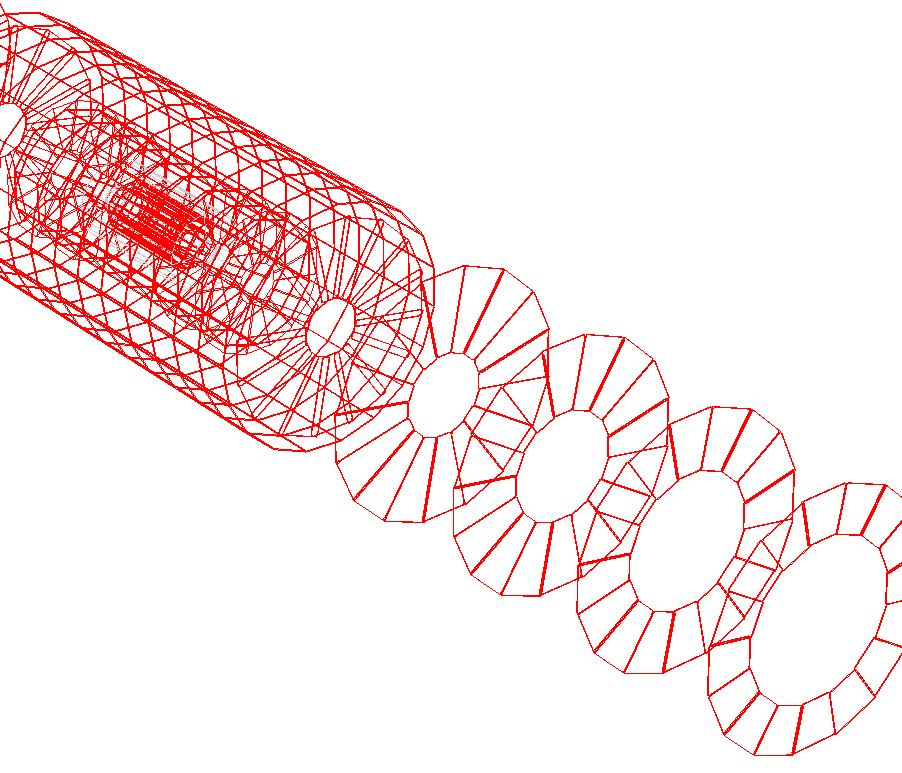
\includegraphics[width=0.5\hsize]{Modelling/fig/ild_inner_trackers_surfaces.png}
\end{tabular}
\caption{\label{fig:inner_trk_surfaces} Left: Inner tracking detectors in the ILD simulation model.
  Right: Surfaces used for track reconstruction, attached to the volumes of the simulation model.}
\end{figure}
%%%%%%%%%%%%%%%%%

\subsection{Particle Flow}

After the reconstruction of charged particle tracks the  \emph{particle flow algorithm} (PFA) is applied
to reconstruct particle showers in the calorimeters.  PFA aims at reconstructing every individual particle
created in the event in order to take the best available measurement for the given type, i.e.:
\begin{itemize}
\item charged particles\\
  using the momentum measured in the tracking detectors with the excellent resolution described in sec.~\ref{sec:system-performance}
\item photons\\
  measured in the Ecal with an energy resolution of $\sigma(E)/E \sim  17\% / \sqrt{(E/\rm{GeV})}$
\item neutral hadrons\\
  measured predominantly in the Hcal\footnote{hadronic showers often start in the Ecal and might extend into the Muon system -
    this is taken into account in PandorPFA} with an energy resolution of $\sigma(E)/E \sim  50\% / \sqrt{(E/\rm{GeV})}$ %%\fix{is this the correct number?}
\end{itemize}

 The best jet energy measurement in hadronic events would be achieved if the above algorithm would work perfectly. However in reality
 there is always confusion in the assignment of individual \emph{CalorimeterHits} to Clusters and showers as well as in the assignment
 of tracks to clusters. The best PFA implementation to date is PandoraPFA~\cite{Marshall:2015rfa}, which is available in iLCSoft and used
 by ILD. The input to PandoraPFA are the reconstructed tracks, candidates for  kinks and  $V0$s as well as all digitized calorimeter hits.
 A number of sophisticated clustering algorithms are the applied in an iterative way, thereby optimizing th track-cluster matching
 based on the momentum-energy consistency.

\subsection{High Level Reconstruction}

After having reconstructed all the individual particles in the event, the next step in the processing is the reconstruction of
primary and secondary vertices. This is carried out in iLCSoft with the LCFIPlus~\cite{Suehara:2015ura} package.
The primary vertex of the event is found in a tear-down procedure taking into account constraints from the expected beam spot
$(\sigma_x=516~\rm{nm}, \sigma_y=7.7~\rm{nm},\sigma_z \sim 200~\mu\rm{m}~~\rm{at}~~~E_{cms}=250~\rm{GeV})$.
In a second step LCFIPlus tries to identify secondary vertices, applying suitable requirements for invariant masses, momentum directions
and $\chi^2$s. Secondary vertices and optionally isolated Leptons can be used by LCFIPlus for jet clustering, aiming at high efficiency for correctly
identifying heavy flavor jets. The actual jet clustering is then performed by using a cone-based clustering with a Durham-like algorithm.
Alternatively users can use $k_T$ jet clustering algorithms from the Fastjet~\cite{Cacciari:2006sm} that is interfaced to Marlin in a dedicated
package MarlinFastJet. LCFIPlus also provides algorithms for jet flavor tagging using boosted decision trees (BDTs) based on suitable
variables from tracks and vertices. A palette of additional high level reconstruction algorithms is used for physics analyses:
\begin{itemize}
\item particle identification using dE/dx, shower shapes and multi-variate methods
\item $\gamma\gamma$-finders for the identification of $\pi^0$s and $\eta$s
\item reconstructed particle to Monte-Carlo truth linker for cross checking analysis and reconstruction efficiencies
\item tools for jet clustering using Monte-Carlo truth information
\item processors for the computation of various event shapes
\end{itemize}



\section{\label{sec:monte-carlo} Monte Carlo Production on the Grid}

The linear collider community uses the ILCDirac~\cite{Grefe:2014sca} toolkit for large scale Monte Carlo production on the Grid.
ILCDirac is highly configurable and ILD uses a dedicated production chain~\cite{Miyamoto:2019xve}, a schematic view of which is shown in Fig.~\ref{fig:sim_ild_mcprod}.
The Monte Carlo production is split into four main steps:
\begin{itemize}
\item GenSplit\\
  Split generator file to many files with small number of event files so that simulation and reconstruction jobs complete in adequate CPU time and 
produce a managable size of output files.  This has the advantage that the same input files can also be used for fast simulation programs such as SGV~\cite{Berggren:2012ar}.
\item Simulation\\
  Simulation of the detector response to the generated particles in the events using ddsim, a python application using the Geant4 gateway DDG4 with
  the detailed detector simulation model.
\item Reconstruction\\
  Full event reconstruction with the algorithms described in sec.~\ref{sec:reco}, writing out detailed \emph{REC}-files with all available information,
  including digitized hits and a much reduced \emph{DST}-file format.
\item{Merging of DST files}\\
  The rather small DST-files are merged into larger files for easier handling.
\end{itemize}
%
In order to investigate the effect reducing the detector dimensions on the physics performance, two large Monte Carlo data sets for the large and small
ILD simulation models have been produced. The produced data sets correspond roughly to $500~\invfb$ at $E_{cms}=500~\GeV$ with the exact numbers of
events processed for the different classes shown in table~\ref{tab:mcprod_evtnum}.

\begin{table}[htbp]
\renewcommand{\arraystretch}{1.25}

\centering\small
\begin{tabular}{lcl}
\hline
 event class  &  description & events processed \\ 
\hline 
2f &   two fermion  final states &  $60.0 \times 10^6$ \\
4f &  four fermion final states & $22.6 \times 10^6$ \\
5f &  five fermion final states & $4.01 \times 10^6$ \\
6f &   six fermion  final states &  $13.8 \times 10^6$ \\
aa\_4f & two fermion by $\gamma\gamma$ interaction & $1.63 \times 10^6$ \\
higgs & higgs process & $3.97 \times 10^6$ \\
np & new physics process & $3.25 \times 10^6$ \\
\hline
aa\_lowpt &  $\Pgamma \Pgamma \to hadrons$ background  &  $2.50 \times 10^6$ \\
seeablepairs &   $\Pep\Pem$-pair background    &  $1.00\times 10^5$ BXs \\
calibration & single particle, $q\bar{q}$ events & $27.71\times 10^6$ \\
\hline
6f(WW) &  dedicated 6f sample at $E_{cms}=1~\TeV$ &  $1.75 \times 10^6$ \\

\hline
\end{tabular}
\caption{Number of Monte Carlo events produced for the different event classes. 
About same number of events were produced for the large and the small ILD simulation model.
Sum of two models are shown in the table.} 
\end{table}


%-----------------------------------------------------------------------

%%%%%%%%%%%%%%%%
\thisfloatsetup{floatwidth=\textwidth,capposition=below}
\begin{figure}[b!]
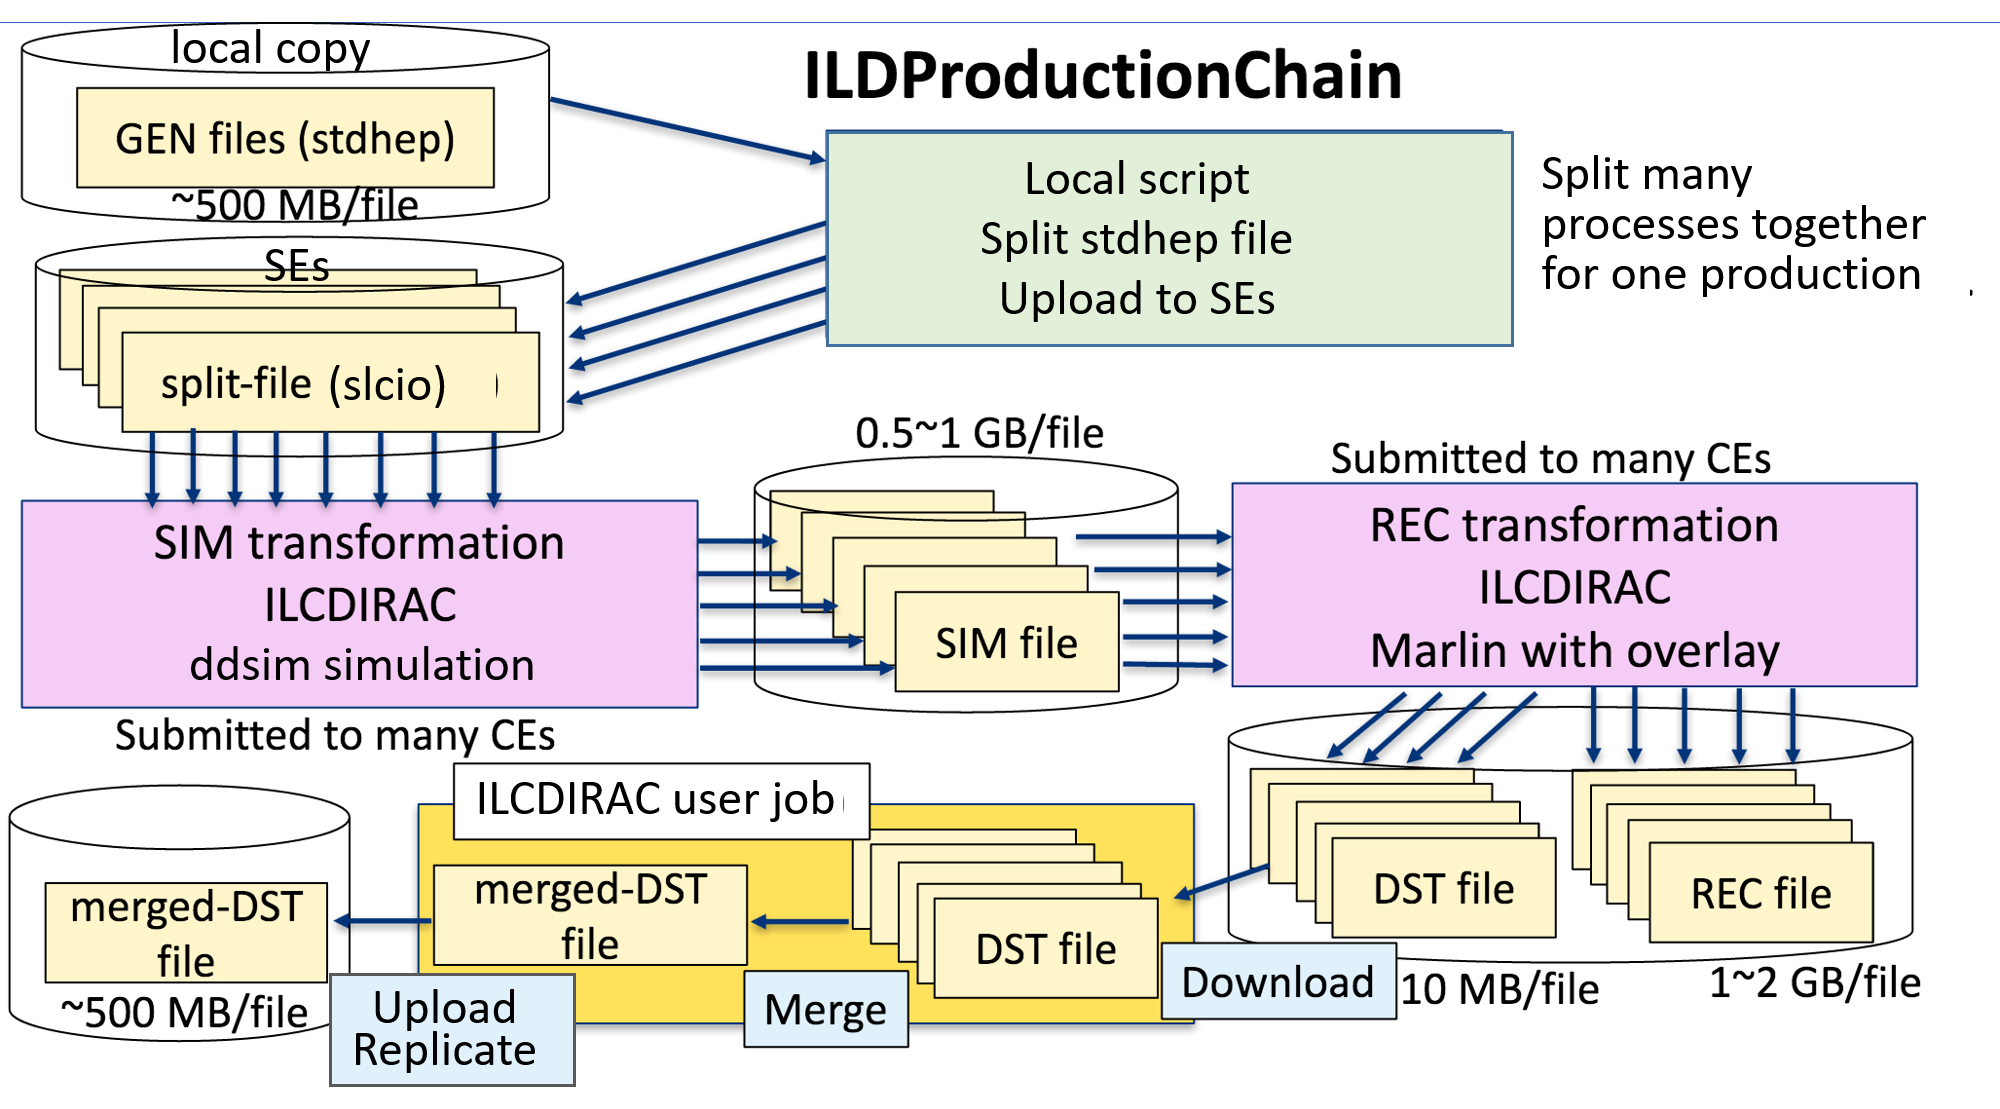
\includegraphics[width=1.0\hsize]{Modelling/fig/ilcdirac_ild_scheme.png}
\caption{\label{fig:sim_ild_mcprod} Schematic view of the Monte Carlo production system used for ILD.}
\end{figure}
%%%%%%%%%%%%%%%%%

